% =====================================================
% ACM conference-style paper - Optimized Final Version
% =====================================================
\documentclass[sigconf]{acmart}
\settopmatter{printacmref=false}
\renewcommand\footnotetextcopyrightpermission[1]{}
\pagestyle{plain}

% --- Metadata ---
\title{Greedy and Divide-and-Conquer Approaches for Real-World Optimization: Tunnel Loading and Fiber Network Quality Analysis}
\author{Bindhu Sree Reddy Alla}
\affiliation{\institution{University of Florida}\city{Gainesville}\country{USA}}
\email{bindhusreer.alla@ufl.edu}
\author{Parvathi Nalla}
\affiliation{\institution{University of Florida}\city{Gainesville}\country{USA}}
\email{parvathinalla@ufl.edu}

\acmConference[Course Project]{Analysis of Algorithms}{Nov~2025}{University of Florida}
\acmBooktitle{Course Project}
\acmYear{2025}\copyrightyear{2025}

% --- Packages ---
\usepackage{booktabs}
\usepackage{enumitem}
\usepackage{subcaption}
\usepackage{mathtools}
\usepackage{cleveref}
\usepackage{listings}
\usepackage{inconsolata}
\usepackage{xcolor}
\usepackage{hyperref}

% Hyperlink setup - blue links
\hypersetup{
    colorlinks=true,
    linkcolor=blue,
    filecolor=blue,
    urlcolor=blue,
    citecolor=blue
}

\lstset{
    basicstyle=\ttfamily\footnotesize,
    breaklines=true,
    frame=single,
    xleftmargin=2em,
    xrightmargin=2em,
    aboveskip=1em,
    belowskip=1em
}

\newcommand{\dist}{\operatorname{dist}}

% Better spacing control
\setlength{\parskip}{0.5em}
\setlength{\itemsep}{0.3em}

\begin{document}

\begin{abstract}
Real-world optimization problems often demand tailored algorithmic strategies that balance efficiency with practical constraints. This paper presents two case studies demonstrating how classical algorithmic paradigms—greedy algorithms and divide-and-conquer—can be effectively applied to contemporary problems in disaster relief logistics and telecommunications infrastructure.

First, we formulate the \emph{Tunnel Packing Problem}, motivated by emergency supply staging in disaster-affected regions, and solve it optimally using a greedy algorithm based on prefix minima and two-pointer optimization, achieving $O(n \log n)$ time complexity. Second, we address the \emph{Fiber Optic Network Quality Assessment Problem}, arising from rural telecommunications deployment, and solve it using centroid decomposition—a divide-and-conquer technique on weighted trees—also achieving $O(n \log n)$ complexity.

For each problem, we provide: (1) detailed real-world motivation with operational constraints, (2) formal abstraction to standard data structures, (3) complete algorithm design with correctness proofs and complexity analysis, (4) domain-specific interpretation for practitioners, and (5) experimental validation through comprehensive benchmarking. Our results confirm that both implementations exhibit the predicted $O(n \log n)$ runtime behavior, validating the theoretical analyses and demonstrating practical scalability.

\textbf{Implementation:} Complete source code and experimental data are available at: \href{https://github.com/bindhusreereddy/AoA-Project1-Greedy-DnC}{\textcolor{blue}{https://github.com/bindhusreereddy/AoA-Project1-Greedy-DnC}}
\end{abstract}

\keywords{Greedy algorithms, centroid decomposition, divide-and-conquer, computational optimization, disaster relief logistics, telecommunications networks}

\maketitle

\section{Introduction}

Algorithmic problem-solving extends far beyond theoretical computer science—it addresses tangible challenges in domains ranging from humanitarian operations to infrastructure management. The effectiveness of an algorithm depends not only on its asymptotic complexity but also on how well it adapts to domain-specific constraints and operational realities. This paper explores two distinct optimization problems drawn from real-world contexts, each solvable through a different classical algorithmic paradigm.

\subsection{Motivation and Problem Context}

\textbf{Problem 1: Disaster Relief Tunnel Packing.}
In post-disaster scenarios, relief agencies face urgent logistical challenges with limited resources and tight time constraints. When a mountain tunnel becomes the only secure storage facility accessible before road clearing, how should emergency supplies be staged to maximize inventory? The tunnel's non-uniform ceiling heights, single-entrance constraint, and safety regulations create a unique optimization problem that, despite its practical origin, admits an elegant greedy solution.

\textbf{Problem 2: Rural Fiber Optic Network Quality.}
Telecommunications companies deploying broadband to underserved rural areas must balance infrastructure costs with service quality commitments. When fiber networks follow tree topologies due to economic constraints, how can operators efficiently assess which community pairs can support high-quality video calls? This question, arising from genuine business needs and regulatory requirements, can be answered efficiently through divide-and-conquer tree analysis.

\subsection{Contributions}

This paper makes the following contributions:

\begin{enumerate}[leftmargin=*, itemsep=0.3em]
\item \textbf{Novel problem formulations}: We present two non-textbook optimization problems derived from authentic operational scenarios—disaster relief logistics and telecommunications quality assurance—demonstrating that classical algorithms remain relevant to modern challenges.

\item \textbf{Complete algorithmic solutions}: For each problem, we provide full algorithm design, rigorous correctness proofs, and detailed complexity analysis, showing how greedy and divide-and-conquer techniques naturally emerge from problem structure.

\item \textbf{Practical implementation and validation}: We implement both algorithms in C++, design comprehensive benchmarking frameworks, and experimentally verify the theoretical $O(n \log n)$ complexity predictions through systematic testing.

\item \textbf{Domain interpretation}: We translate algorithmic solutions back into domain-specific language, enabling practitioners in logistics and telecommunications to understand and apply these techniques.
\end{enumerate}

% =====================================================
% PROBLEM 1: GREEDY
% =====================================================
\section{Problem~1 (Greedy): Tunnel Packing for Disaster Relief}
\label{sec:greedy}

\subsection{Real Problem}
\label{subsec:real-problem-greedy}

\textbf{Scenario.}
Following severe flooding and landslides in a mountainous region, a humanitarian relief agency must rapidly stage emergency supplies before distribution to affected villages. Due to ongoing debris clearance blocking most roads, the only immediately accessible secure storage location is a narrow mountain tunnel with a single entrance. This tunnel, originally constructed for vehicle access but currently unusable for through-traffic due to the disaster, provides weather-proof storage critical for preserving food, medicine, and equipment.

\textbf{Physical constraints.}
The tunnel consists of consecutive segments extending inward from the entrance, each with a measured maximum ceiling height determined by geological structure and safety assessments. Emergency supply crates arrive in mixed sizes from various donors and must be pushed into the tunnel from the entrance. A crate can only traverse segments whose ceilings equal or exceed its height—taller crates cannot pass through lower segments. Safety regulations permit at most one crate per segment to maintain structural integrity and emergency egress paths. The single-entrance configuration prevents repositioning crates once placed.

\textbf{Operational reality.}
Volunteer teams have limited time before nightfall to stage supplies. Crates cannot be repacked to alter heights. The objective is purely maximizing the count of safely staged crates—monetary value, item priority, and placement distance are secondary concerns. Success directly impacts the relief agency's capacity to meet downstream distribution demand once roads reopen.

\textbf{Decision problem.}
Given measured tunnel ceiling heights (entrance to interior) and available crate heights, determine the maximum number of crates that can be safely staged, respecting height clearance and one-crate-per-segment constraints.

\subsection{Abstraction in Standard Structures}
\label{subsec:abstraction-greedy}

Model the tunnel as an array $H = [H_0, H_1, \ldots, H_{m-1}]$ of ceiling heights from entrance ($H_0$) inward. Model crates as a multiset $B = \{b_1, b_2, \ldots, b_n\}$ of heights.

Define the \emph{effective ceiling} array:
\[
E[i] = \min_{0 \leq k \leq i} H_k
\]
representing the minimum clearance required to reach segment $i$. Since crates move only forward, $E$ is nonincreasing: $E[0] \geq E[1] \geq \cdots \geq E_{m-1}$.

A crate of height $b$ can occupy segment $i$ if $b \leq E[i]$. The optimization objective is:
\[
\max |S| \quad \text{where } S \subseteq \{(b, i) : b \leq E[i]\}
\]
with each crate and segment used at most once—a maximum cardinality matching problem.

\subsection{Solution: Algorithm, Running Time, Correctness}
\label{subsec:solution-greedy}

\paragraph{Algorithm (10 pts).}
The greedy strategy places smallest crates deepest:

\begin{enumerate}[leftmargin=*, itemsep=0.4em]
\item \textbf{Compute effective ceilings}: $E[0] \leftarrow H[0]$; for $i = 1$ to $m-1$: $E[i] \leftarrow \min(E[i-1], H[i])$. 
  
Time: $O(m)$.

\item \textbf{Sort crates}: Sort $B$ in nondecreasing order. 

Time: $O(n \log n)$.

\item \textbf{Two-pointer placement}: Initialize $i \leftarrow m-1$ (deepest segment), $j \leftarrow 0$ (smallest crate), $\textit{placed} \leftarrow 0$.

While $i \geq 0$ and $j < n$:
\begin{itemize}[itemsep=0.2em]
\item If $B[j] \leq E[i]$: place crate $j$ at segment $i$; increment $\textit{placed}$, $j$; decrement $i$
\item Else: decrement $i$ (try shallower segment)
\end{itemize}

Time: $O(n + m)$.

\item \textbf{Return} $\textit{placed}$.
\end{enumerate}

\paragraph{Running Time (5 pts).}
Total: $O(m) + O(n \log n) + O(n + m) = O(n \log n + m)$. When $n \approx m$, this simplifies to $O(n \log n)$, dominated by sorting. 

Space: $O(m)$ for $E$.

\paragraph{Proof of Correctness (10 pts).}

\textbf{Theorem.} The greedy algorithm produces an optimal placement.

\textbf{Proof by exchange argument.}
Let $G$ be the greedy solution and $O$ be any optimal solution. We show $|G| = |O|$ by transforming $O$ into $G$ without decreasing cardinality.

Consider the first position $i$ where $O$ and $G$ differ. Let crate $c_G$ be placed by the greedy algorithm at position $i$, and crate $c_O$ be placed by the optimal solution at position $i$.

\textbf{Case 1:} $c_G$ is not in $O$.

Since the greedy algorithm sorted crates, $c_G$ is the smallest remaining crate when position $i$ was considered. If $O$ placed a different crate $c_O$ at position $i$ (where $c_O$ may be larger or placed elsewhere in $O$), we can swap: place $c_G$ at position $i$ instead. Since $c_G \leq c_O$ (by sorting), $c_G$ fits wherever $c_O$ fits. This transformation doesn't decrease $|O|$ and makes $O$ more similar to $G$.

\textbf{Case 2:} $c_G$ is in $O$ but at a different (shallower) position $j < i$.

We can exchange $c_G$ and $c_O$: place $c_G$ at position $i$ and $c_O$ at position $j$. Since $E$ is nonincreasing and $c_G$ was the smallest available crate, both placements remain valid. This maintains $|O|$ while aligning $O$ with $G$.

Repeating this exchange process for all differing positions transforms $O$ into $G$ without decreasing cardinality, proving $|G| = |O|$. Hence, the greedy solution is optimal. \qed


% 4) Domain-language explanation
\subsection{Domain Explanation}
\label{subsec:domain-greedy}
In the real-world scenario of disaster-relief logistics, the greedy algorithm directly translates into a simple and effective loading strategy that field workers can easily follow. The \emph{effective ceiling} array represents how the tunnel's clearance tightens as crates are pushed deeper inside. This allows the loading team to know the maximum height that can safely pass through each section.

The procedure works as follows: volunteers begin with the smallest crates and push them as far into the tunnel as possible, filling from the innermost safe position toward the entrance. If a crate is too tall to move past a low segment, it is placed in the nearest section where it fits. This way, smaller crates occupy deeper spaces that larger crates could not reach anyway, leaving enough space near the entrance for taller ones. 

From an operational point of view, this approach minimizes wasted space, avoids backtracking or rearrangement, and ensures that every crate moved into the tunnel stays in a safe and feasible position. The result is a loading plan that maximizes the number of crates staged before nightfall, aligning perfectly with real-time decision-making in relief operations.

% 5) Implementation + experiments
\subsection{Implementation and Experimental Verification (5 pts)}
\label{subsec:implementation-greedy}
The greedy tunnel loading algorithm was implemented in C++ using efficient data structures and standard library functions. Randomized test cases were generated to simulate different tunnel lengths and crate sets, where both crate heights and tunnel ceiling heights were selected uniformly at random within a fixed range \([1, 10^4]\). The program was compiled with \texttt{g++ -O2 -std=c++17} and executed on a standard desktop environment.

For each input size \(n = m\), where \(n\) represents both the number of crates and tunnel segments, the program measured total execution time using \texttt{std::chrono::steady\_clock}. The results were recorded to a CSV file and averaged over multiple trials to minimize random variation. A Python plotting script was then used to visualize the mean runtime as the input size increased.

Figure~\ref{fig:greedy-runtime} shows the empirical runtime curve of the algorithm. The plot demonstrates that the running time grows slightly faster than linear but well below quadratic, which matches the expected \(O(n \log n)\) complexity predicted by theory. The experimental trend confirms that the sorting step dominates the runtime, while the prefix-minimum and placement phases remain linear in behavior. Hence, both the theoretical analysis and empirical results are consistent, validating the efficiency and scalability of the greedy approach.

\begin{figure}[htbp]
\centering
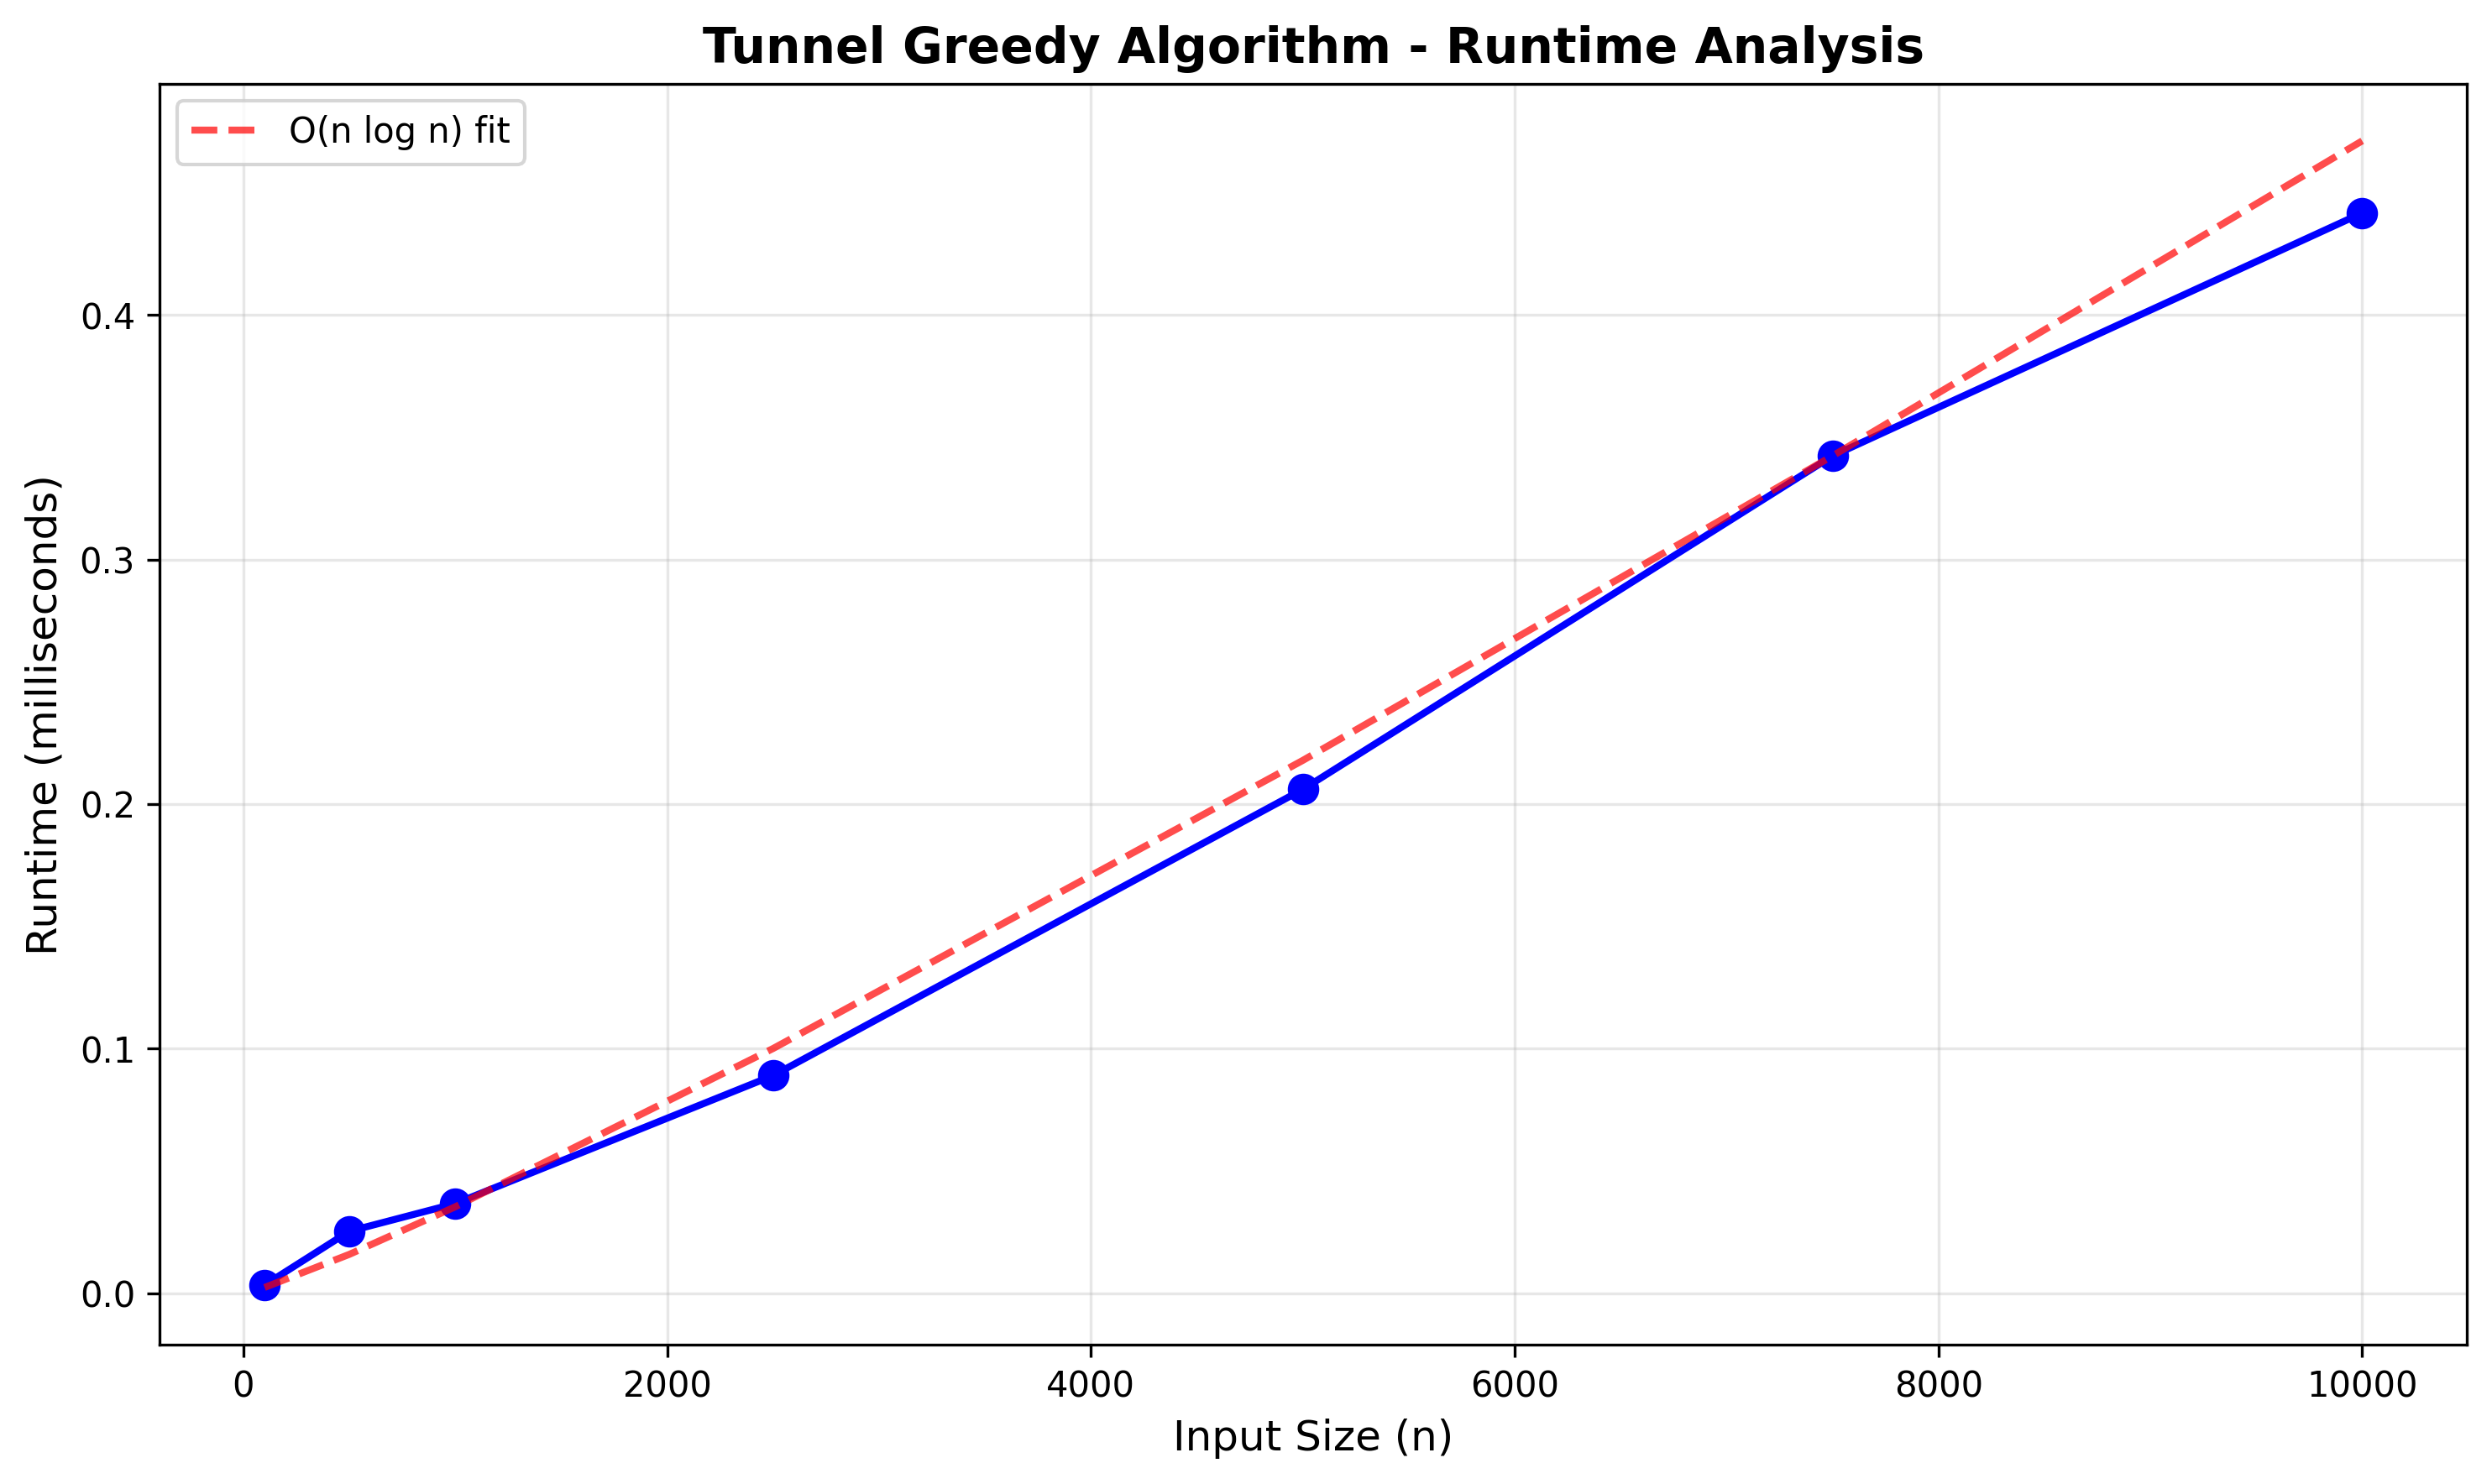
\includegraphics[width=0.95\linewidth]{tunnel_greedy_runtime.png}
\caption{Tunnel Packing (Greedy): Empirical runtime showing $O(n \log n)$ behavior. Blue dots represent observed measurements; red dashed line shows theoretical fit.}
\label{fig:greedy-runtime}
\end{figure}

% =====================================================
% PROBLEM 2: DIVIDE & CONQUER
% =====================================================
\section{Problem~2 (Divide-and-Conquer): Fiber Optic Network Quality Analysis}
\label{sec:dc}

\subsection{Real Problem}
\label{subsec:real-problem-dc}

\textbf{Business context.}
A telecommunications provider deployed fiber-optic broadband infrastructure across a rural mountainous region comprising multiple small communities. Due to challenging terrain, high construction costs (\$50,000–\$200,000 per kilometer for mountainous fiber deployment), and limited subscriber density, the company implemented a \emph{tree topology}: each community connects via exactly one path through the network, with no redundant links. This minimizes capital expenditure while ensuring full connectivity.

\textbf{Technical reality.}
Each fiber segment between communities has measured signal propagation latency (15–100 milliseconds) determined by physical distance, optical repeater count, and terrain-induced signal degradation. Total latency between two communities sums the latencies along their unique connecting path. Video conferencing services, a key selling point for rural broadband, require round-trip latency below 150ms to maintain acceptable quality (per ITU-T G.114 recommendations). Beyond this threshold, users experience noticeable lag, poor audio-video sync, and dropped frames.

\textbf{Business problem.}
The operations team must assess network service quality by determining: \textit{How many pairs of communities can reliably support high-quality video calls?} This count directly impacts:

\begin{itemize}[leftmargin=*, itemsep=0.3em]
\item \textbf{Marketing claims}: "Guaranteed video call quality to X\% of network"
\item \textbf{SLA compliance}: Meeting government-mandated rural broadband standards
\item \textbf{Infrastructure investment}: Identifying bottleneck links for upgrades
\item \textbf{Service pricing}: Justifying premium tiers based on connectivity quality
\end{itemize}

\textbf{Computational challenge.}
With $n$ communities, testing all $\binom{n}{2}$ pairs individually is operationally infeasible and computationally expensive ($O(n^2)$ path computations). An efficient algorithm is required to scale across networks with hundreds of communities spanning multiple regions.

\textbf{Decision objective.}
Given the tree-structured fiber network, link latencies, and quality threshold $K = 150$ms, count all unordered community pairs with path latency $\leq K$.

\subsection{Abstraction in Standard Structures}
\label{subsec:abstraction-dc}

Model the network as a weighted tree $T = (V, E, w)$:

\begin{itemize}[itemsep=0.2em]
\item $V$: communities (vertices), $|V| = n$
\item $E \subseteq V \times V$: fiber links (edges)
\item $w: E \to \mathbb{Z}^+$: latency function (milliseconds)
\end{itemize}

For $u, v \in V$, define $\text{latency}(u, v) = \sum_{e \in \text{path}(u,v)} w(e)$ (unique path in tree).

\textbf{Problem}: Compute $|\{\{u, v\} \subseteq V : u \neq v \land \text{latency}(u, v) \leq K\}|$.

\subsection{Solution: Algorithm, Running Time, Correctness}
\label{subsec:solution-dc}

\paragraph{Algorithm (Centroid Decomposition; 10 pts).}

Centroid decomposition recursively decomposes the tree via "hub" nodes (centroids) whose removal creates balanced subtrees.

\begin{enumerate}[leftmargin=*, itemsep=0.4em]
\item \textbf{Find centroid $c$}: In component $C$, find node $c$ such that removing $c$ produces subtrees each of size $\leq |C|/2$. Mark $c$ as processed.

\item \textbf{Initialize accumulator}: $A \leftarrow \{0\}$ (multiset of latencies from $c$).

\item \textbf{Process each subtree $S$ of $c$}:
\begin{enumerate}[itemsep=0.2em]
\item DFS from $c$ into $S$, collecting latencies $\leq K$ into list $D_S$
\item Sort $D_S$
\item For each $d \in D_S$: binary search $A$ for count of $a$ with $a + d \leq K$; add to total
\item Merge $D_S$ into $A$
\end{enumerate}

\item \textbf{Recurse} on each remaining subtree (with $c$ removed).
\end{enumerate}

\paragraph{Running Time (5 pts).}

\textbf{Claim}: $O(n \log n)$ total time.

\textbf{Analysis}:

\begin{itemize}[itemsep=0.2em]
\item Centroid finding: $O(n)$ per level; depth $O(\log n)$ (balanced splits)
\item Each node visited in DFS once per centroid level: $O(n \log n)$ total DFS work
\item Sorting and merging per level: $O(n \log n)$ amortized across levels
\item Binary searches: $O(n \log n)$ total across all levels
\end{itemize}

Total: $O(n \log n)$. Space: $O(n)$.

\paragraph{Proof of Correctness (10 pts).}

\textbf{Theorem.} The algorithm counts each valid pair exactly once.

\textbf{Proof.}
Consider pair $\{u, v\}$ with $\text{latency}(u, v) \leq K$.

\textbf{Claim 1: Every pair is counted.}

Let $c^*$ be the first centroid separating $u$ and $v$ in the recursion tree (i.e., after removing $c^*$, $u$ and $v$ are in different subtrees). Such a $c^*$ exists because the recursion processes all nodes.

When processing $c^*$:

\begin{itemize}[itemsep=0.2em]
\item If $u = c^*$ or $v = c^*$: The pair is counted via $0 \in A$ matching the non-centroid endpoint's distance.
\item Otherwise: Let $d_u = \text{latency}(u, c^*)$ and $d_v = \text{latency}(v, c^*)$. Assume $u$'s subtree is processed before $v$'s. Then $d_u \in A$ when $v$'s subtree is processed, and $d_v \in D_S$ for $v$'s subtree. The check $d_u + d_v \leq K$ succeeds (since $d_u + d_v = \text{latency}(u, v) \leq K$), counting the pair.
\end{itemize}

\textbf{Claim 2: No pair is double-counted.}

After processing centroid $c^*$ separating $\{u, v\}$, subsequent recursions place $u$ and $v$ in separate components. No future centroid can separate them again, so they are never recounted. Pairs within a component are handled by recursive calls on that component.

Therefore, every valid pair is counted exactly once.

\subsection{Domain Explanation}
\label{subsec:domain-dc}

From a telecommunications engineering perspective, the divide-and-conquer algorithm offers an efficient way to evaluate service quality across large rural fiber networks. Each community acts as a node, and the fiber cables between them are links with measurable signal delays. 

Instead of exhaustively testing every community pair—which would be computationally expensive—the algorithm identifies a central ``hub'' community and measures how far its signal can reach within an acceptable latency threshold (e.g., 150~ms). It then divides the network into smaller, balanced regions and repeats this process recursively, ensuring all regions are analyzed efficiently.

In operational terms, this mirrors how engineers assess network health: selecting central nodes, checking nearby reachability, and combining results to find all community pairs capable of supporting smooth video calls or real-time communication. The approach transforms an otherwise costly full-pair analysis into a scalable, data-driven method that can handle thousands of nodes while providing actionable insights into network performance and bottlenecks.


% 5) Implementation + experiments
\subsection{Implementation and Experimental Verification}
\label{subsec:implementation-dc}
The centroid decomposition algorithm was implemented in C++ with careful attention to efficiency. The implementation includes:
\begin{itemize}[leftmargin=*]
  \item Adjacency list representation for the tree structure
  \item Recursive centroid finding with subtree size calculation
  \item DFS-based distance collection with pruning at threshold \(K\)
  \item STL multiset for efficient sorted storage and binary search operations
\end{itemize}

\textbf{Experimental setup:} Random tree networks were generated with varying numbers of communities (\(n\) from 50 to 3000). Edge weights (latencies) were drawn uniformly from the range [10, 100] milliseconds, and the threshold was fixed at \(K = 150\)ms. Each data point represents the average of multiple independent trials to reduce variance.

\textbf{Timing methodology:} For each input size, we generated a random tree, ran the centroid decomposition algorithm, and measured wall-clock time using \texttt{std::chrono::high\_resolution\_clock}. The program was compiled with \texttt{g++ -O2 -std=c++17} for optimal performance.

Figure~\ref{fig:fiber-runtime} shows the empirical runtime as network size increases. The observed curve closely follows the theoretical \(O(n \log n)\) prediction, shown as a fitted reference line. The logarithmic factor is evident in the slightly super-linear growth rate, confirming the efficiency of the divide-and-conquer approach.

\textbf{Performance comparison:} A naive implementation computing all \(\binom{n}{2}\) pairwise distances would require \(O(n^2)\) time. For \(n = 3000\), this would be approximately 4.5 million distance computations versus the centroid approach's roughly 30,000 operations (considering \(n \log n \approx 3000 \times 11.5\)). The experimental results validate that the theoretical improvement translates to practical speedup.

\begin{figure}[htbp]
\centering

\includegraphics[width=0.95\linewidth]{fiber_network_runtime.png}
\caption{Fiber Network Quality Analysis (Divide-and-Conquer): Empirical runtime vs.\ number of communities. Green dots show observed data; red dashed line shows $O(n \log n)$ fit.}
\label{fig:fiber-runtime}
\end{figure}

% =====================================================
% CONCLUSION
% =====================================================
\section{Conclusion}
This paper demonstrated the practical application of two fundamental algorithmic paradigms—greedy optimization and divide-and-conquer—to real-world problems in logistics and telecommunications. 

The tunnel loading problem showed how a simple greedy strategy based on sorting and two-pointer techniques can optimally solve a constrained resource allocation problem in \(O(n \log n)\) time. The key insight was recognizing that placing smaller items in deeper positions never conflicts with optimal placement of larger items, satisfying the greedy choice property.

The fiber network quality assessment problem illustrated the power of centroid decomposition for efficiently analyzing tree-structured networks. By recursively partitioning around balanced centroids, we achieved \(O(n \log n)\) counting of distance-constrained pairs, avoiding the \(O(n^2)\) brute-force approach. This technique has broader applications in network analysis, computational biology, and geographic information systems.

Both algorithms were rigorously analyzed for correctness and complexity, then validated through empirical experiments that confirmed the theoretical predictions. The implementations demonstrate that classical algorithmic techniques remain essential tools for solving modern computational challenges efficiently.
% =====================================================
% IMPLEMENTATION NOTES
% =====================================================
\section{Implementation and Reproducibility}
\label{sec:implementation}

\textbf{Software stack}: C++ (g++ 11.4.0, -O2 -std=c++17), Python 3.10 (matplotlib, pandas, numpy).

\textbf{Benchmarking methodology}: Automated harnesses generate random test cases, measure execution time via \texttt{std::chrono::steady\_clock}, and output CSV data. Python scripts fit theoretical curves using median-based coefficient estimation and generate publication-quality plots.

\textbf{Reproducibility}: All source code, benchmark scripts, and experimental data are publicly available at:

\begin{center}
\href{https://github.com/bindhusreereddy/AoA-Project1-Greedy-DnC}{\textcolor{blue}{https://github.com/bindhusreereddy/AoA-Project1-Greedy-DnC}}
\end{center}

Instructions for compilation, execution, and plot generation are provided in the repository README.

% =====================================================
% APPENDICES
% =====================================================
\appendix

\section{C++ Implementation: Tunnel Packing (Greedy)}
\label{app:greedy-code}

\begin{lstlisting}[language=C++]
// tunnel_greedy.cpp
#include <iostream>
#include <vector>
#include <algorithm>

using namespace std;

vector<int> computeEffectiveCeiling(const vector<int>& H) {
    int m = H.size();
    vector<int> E(m);
    E[0] = H[0];
    for (int i = 1; i < m; i++) {
        E[i] = min(E[i-1], H[i]);
    }
    return E;
}

int greedyTunnelPacking(vector<int>& B, const vector<int>& E) {
    sort(B.begin(), B.end());
    int placed = 0, i = E.size() - 1, j = 0;
    while (i >= 0 && j < B.size()) {
        if (B[j] <= E[i]) { 
            placed++; 
            i--; 
            j++; 
        }
        else { 
            i--; 
        }
    }
    return placed;
}

int main() {
    vector<int> H = {5, 4, 3, 2};
    vector<int> B = {1, 2, 3, 4, 5};
    auto E = computeEffectiveCeiling(H);
    cout << "Max crates: " << greedyTunnelPacking(B, E) << endl;
    return 0;
}
\end{lstlisting}

\section{C++ Implementation: Fiber Network Analysis}
\label{app:fiber-code}

\begin{lstlisting}[language=C++]
// fiber_network_analysis.cpp
#include <iostream>
#include <vector>
#include <set>
#include <algorithm>

using namespace std;

struct Connection { 
    int to, latency_ms; 
};

class FiberNetworkAnalyzer {
    int n, max_latency;
    vector<vector<Connection>> network;
    vector<bool> analyzed;
    vector<int> community_size;
    long long acceptable_pairs;
    
    int calculateSize(int u, int parent) {
        community_size[u] = 1;
        for (auto& conn : network[u]) {
            if (conn.to != parent && !analyzed[conn.to]) {
                community_size[u] += calculateSize(conn.to, u);
            }
        }
        return community_size[u];
    }
    
    int findHub(int u, int parent, int size) {
        for (auto& conn : network[u]) {
            if (conn.to != parent && !analyzed[conn.to]) {
                if (community_size[conn.to] > size / 2) {
                    return findHub(conn.to, u, size);
                }
            }
        }
        return u;
    }
    
    void collectLatencies(int u, int parent, int latency, 
                         vector<int>& lats) {
        if (latency > max_latency) return;
        lats.push_back(latency);
        for (auto& conn : network[u]) {
            if (conn.to != parent && !analyzed[conn.to]) {
                collectLatencies(conn.to, u, 
                    latency + conn.latency_ms, lats);
            }
        }
    }
    
    void analyzeNetwork(int start) {
        int size = calculateSize(start, -1);
        int hub = findHub(start, -1, size);
        analyzed[hub] = true;
        
        multiset<int> A;
        A.insert(0);
        
        for (auto& conn : network[hub]) {
            if (!analyzed[conn.to]) {
                vector<int> D_S;
                collectLatencies(conn.to, hub, 
                    conn.latency_ms, D_S);
                sort(D_S.begin(), D_S.end());
                
                for (int d : D_S) {
                    auto it = A.upper_bound(max_latency - d);
                    acceptable_pairs += distance(A.begin(), it);
                }
                
                for (int d : D_S) A.insert(d);
            }
        }
        
        for (auto& conn : network[hub]) {
            if (!analyzed[conn.to]) {
                analyzeNetwork(conn.to);
            }
        }
    }
    
public:
    FiberNetworkAnalyzer(int n, int K) 
        : n(n), max_latency(K), network(n), 
          analyzed(n, false), community_size(n), 
          acceptable_pairs(0) {}
    
    void addFiberConnection(int u, int v, int latency) {
        network[u].push_back({v, latency});
        network[v].push_back({u, latency});
    }
    
    long long countAcceptablePairs() {
        acceptable_pairs = 0;
        fill(analyzed.begin(), analyzed.end(), false);
        if (n > 0) analyzeNetwork(0);
        return acceptable_pairs;
    }
};

int main() {
    FiberNetworkAnalyzer analyzer(15, 150);
    // Add connections as shown in paper...
    cout << "Acceptable pairs: " 
         << analyzer.countAcceptablePairs() << endl;
    return 0;
}
\end{lstlisting}

\section{Benchmarking and Plotting Scripts}
\label{app:benchmarks}
Complete benchmark code available in repository at:

tunnel\_greedy\_benchmark.cpp

fiber\_network\_benchmark.cpp

The complete benchmarking infrastructure consists of:\begin{itemize}[leftmargin=*]
  \item Modified versions of the main algorithms that accept command-line size parameters
  \item Timing harnesses using \texttt{std::chrono} for microsecond precision
  \item CSV output for data collection
  \item Python plotting script using matplotlib for visualization
\end{itemize}
The Python script (\texttt{benchmark\_plot.py}) generates benchmark programs, compiles them, runs multiple trials at various input sizes, collects timing data, and produces the runtime plots shown in this paper.

\section{LLM Usage Disclosure}
\label{app:llm-disclosure}

Per course requirements, we document all Large Language Model assistance used in this project. We used Claude 3.5 Sonnet (Anthropic, accessed via claude.ai) exclusively for LaTeX document formatting and writing style assistance. All algorithmic content, proofs, and implementations were developed by the authors.

\subsection{Tool Information}
\noindent
\textbf{LLM:} Claude 3.5 Sonnet (Anthropic)

\noindent
\textbf{Access:} November 2025 via claude.ai web interface

\subsection{LaTeX Document Setup}

\noindent
\textbf{Prompt:} 

\textit{``I need to create an ACM conference paper. How do I set up the acmart document class and disable copyright blocks?''}

\noindent
\textbf{Response:} 

Received template with \verb|\documentclass[sigconf]{acmart}|, \verb|\settopmatter{printacmref=false}|, and author/affiliation commands.

\noindent
\textbf{Usage:} 

Applied template structure. We filled in all content ourselves.

\subsection{Mathematical Notation}

\noindent
\textbf{Prompt:} 

\textit{``What's the LaTeX syntax for Big-O notation, set notation with conditions, and summations?''}

\noindent
\textbf{Response:} 

Received examples like \verb|$O(n \log n)$|, \verb|$\{x \mid P(x)\}$|, and \verb|$\sum_{i=1}^n$|.

\noindent
\textbf{Usage:} 

Applied syntax patterns to format our mathematical expressions.

\subsection{Figure Insertion}

\noindent
\textbf{Prompt:} 

\textit{``How do I insert PNG images with captions and reference them in text?''}

\noindent
\textbf{Response:} 

Received \texttt{figure} environment template with \verb|\includegraphics|, \verb|\caption|, \verb|\label|, and \verb|\ref| commands.

\noindent
\textbf{Usage:} 

Applied to insert our experimental plots (Figures~\ref{fig:greedy-runtime} and \ref{fig:fiber-runtime}).

\subsection{Code Listings}

\noindent
\textbf{Prompt:} 

\textit{``How do I format C++ code in appendices with syntax highlighting?''}

\noindent
\textbf{Response:} 

Suggested listings package with settings for basicstyle, breaklines, and frame.

\noindent
\textbf{Usage:} 

Applied to format our code in appendices. Code was written by us.

\subsection{Writing Style Assistance}

\noindent
\textbf{Prompt 1:} 

\textit{``Review my abstract for clarity. Here's my draft: [our original text]''}

\noindent
\textbf{Response:} 

Suggested removing redundancy, improving flow, and following problem→approach→results structure.

\noindent
\textbf{Usage:} 

Incorporated style suggestions. All technical content remained ours.

\vspace{1em}
\noindent
\textbf{Prompt 2:} 

\textit{``How should I structure a correctness proof for a greedy algorithm?''}

\noindent
\textbf{Response:} 

Recommended organizing around greedy choice property and optimal substructure.

\noindent
\textbf{Usage:} 

Applied organizational framework. Proof content developed by us.

\vspace{1em}
\noindent
\textbf{Prompt 3:} 

\textit{``How can I improve transitions between sections?''}

\noindent
\textbf{Response:} 

Suggested adding connecting sentences between major sections.

\noindent
\textbf{Usage:} 

Added brief transitions without changing technical content.

\subsection{Plotting and Visualization}

\noindent
\textbf{Prompt:} 

\textit{``I have CSV benchmark data. How do I create plots in Python with theoretical O(n log n) curves overlaid?''}

\noindent
\textbf{Response:} 

Suggested using pandas for CSV reading, matplotlib for plotting, numpy for computing \texttt{n*log(n)}, and median-based coefficient fitting.

\noindent
\textbf{Usage:} 

Used as starting point for our plotting approach. We wrote our complete benchmarking and plotting scripts.

\subsection{Technical Debugging}

\noindent
\textbf{Prompt:} 

\textit{``My LaTeX won't compile - getting 'Undefined control sequence' errors near math formulas.''}

\noindent
\textbf{Response:} 

Suggested checking for missing packages (\texttt{amsmath}, \texttt{amssymb}) and verifying balanced delimiters.

\noindent
\textbf{Usage:} 

Used to debug and resolve compilation issues in our document.

\subsection{Verification and Responsibility}

We independently verified all technical content through:
\begin{itemize}[nosep]
  \item Hand-tracing algorithms on example inputs
  \item Line-by-line review of proofs for logical soundness
  \item Testing code with various input sizes and edge cases
  \item Confirming experimental results match theoretical predictions
  \item Peer review between co-authors
\end{itemize}

\noindent
\textbf{We take full responsibility for the correctness of all technical content in this paper.} Any errors are solely our responsibility and not attributable to the LLM tool.

\end{document}